\let\negmedspace\undefined
\documentclass{beamer}
\mode<presentation>
\usepackage{amsmath,amssymb,amsfonts,amsthm}
\usepackage{algorithmic}
\usepackage{graphicx}
\usepackage{xcolor}
\usepackage{listings}
\usepackage{mathtools}
\usepackage{tikz}
\usepackage{tcolorbox}
\usepackage{url}

% Custom delimiter commands
\providecommand{\brak}[1]{\ensuremath{\left(#1\right)}}
\providecommand{\sbrak}[1]{\ensuremath{\left[#1\right]}}

% Other useful macros
\newcommand{\myvec}[1]{\ensuremath{\begin{pmatrix}#1\end{pmatrix}}}

\usetheme{Madrid}
\usecolortheme{lily}

\setbeamertemplate{navigation symbols}{}

\numberwithin{equation}{section}

\title{10.3.5.4.3}
\author{EE24BTECH11018 - Durgi Swaraj Sharma}
\date{}

\begin{document}

\frame{\titlepage}

%------------------------------------------------
\begin{frame}
\frametitle{Question}
\textbf{Problem Statement:}

Yash scored $40$ marks in a test, getting $3$ marks for each right answer and losing $1$ mark for each wrong answer. Had $4$ marks been awarded for each correct answer and $2$ marks been deducted for each incorrect answer, then Yash would have scored $50$ marks. How many questions were there in the test?
\end{frame}

%------------------------------------------------
\begin{frame}
\frametitle{Mathematical Formulation}
Let 
\begin{itemize}
    \item $x =$ number of correct answers,
    \item $y =$ number of incorrect answers.
\end{itemize}
Then, we can write the two scenarios as:
\begin{align}
3x - y &= 40, \\
4x - 2y &= 50.
\end{align}
Our goal is to find $x+y$, the total number of questions.
\end{frame}

%------------------------------------------------
\begin{frame}
\frametitle{Matrix Representation}
We represent the system above in matrix form:
\begin{align}
\myvec{3 & -1\\ 4 & -2}\,\myvec{x \\ y} = \myvec{40 \\ 50}.
\end{align}
\end{frame}

%------------------------------------------------
\begin{frame}
\frametitle{LU Decomposition Overview}
Any non-singular matrix $A$ can be decomposed as:
\begin{align}
A = LU,
\end{align}
where:
\begin{itemize}
    \item $L$ is a lower triangular matrix,
    \item $U$ is an upper triangular matrix.
\end{itemize}
Thus, we have:
\begin{align}
A\,\myvec{x \\ y} = LU\,\myvec{x \\ y} = \vec{b}.
\end{align}
\end{frame}

%------------------------------------------------
\begin{frame}
\frametitle{Finding $U$ via Row Reduction}
Consider the coefficient matrix
\begin{align}
A = \myvec{3 & -1\\ 4 & -2}.
\end{align}
To form $U$, we eliminate the subdiagonal element in the second row by performing the row operation:
\begin{align}
R_2 \rightarrow R_2 - \frac{4}{3}R_1.
\end{align}
This yields:
\begin{align}
U = \myvec{3 & -1\\ 0 & -\frac{2}{3}}.
\end{align}
\end{frame}

%------------------------------------------------
\begin{frame}
\frametitle{Constructing $L$}
The lower triangular matrix $L$ captures the multipliers used in the row operations. Since the multiplier is
\begin{align}
l_{21} = \frac{4}{3},
\end{align}
we set
\begin{align}
L = \myvec{1 & 0\\ \frac{4}{3} & 1}.
\end{align}
Thus, the LU decomposition of $A$ is:
\begin{align}
A = \myvec{1 & 0\\ \frac{4}{3} & 1}\,\myvec{3 & -1\\ 0 & -\frac{2}{3}}.
\end{align}
\end{frame}

%------------------------------------------------
\begin{frame}
\frametitle{Doolittle's Algorithm (Overview)}
An alternative method is Doolittle's Algorithm which provides update equations:

\textbf{For $U$:} For each column $j$,
\begin{align}
U_{ij} = 
\begin{cases}
A_{ij} & \text{if } i=1,\\[0.5ex]
A_{ij} - \displaystyle\sum_{k=1}^{i-1} L_{ik}U_{kj} & \text{if } i>1.
\end{cases}
\end{align}

\textbf{For $L$:} For each row $i$,
\begin{align}
L_{ij} = 
\begin{cases}
\frac{A_{ij}}{U_{jj}} & \text{if } j=i,\\[0.5ex]
\frac{A_{ij} - \displaystyle\sum_{k=1}^{j-1} L_{ik}U_{kj}}{U_{jj}} & \text{if } j<i.
\end{cases}
\end{align}
This process decomposes any non-singular matrix $A$ into $L$ and $U$.
\end{frame}

%------------------------------------------------
\begin{frame}
\frametitle{Solving the System via LU Decomposition}
We now solve:
\begin{align}
LU\,\myvec{x \\ y} = \myvec{40 \\ 50}.
\end{align}
This involves two steps:
\begin{enumerate}
    \item Solve $L\,\vec{y} = \vec{b}$ for $\vec{y}$,
    \item Solve $U\,\vec{x} = \vec{y}$ for $\vec{x}$ by back-substitution.
\end{enumerate}
Substitute the known values:
\begin{align}
L\,\myvec{y_1 \\ y_2} &= \myvec{1 & 0\\ \frac{4}{3} & 1}\,\myvec{y_1 \\ y_2} = \myvec{40 \\ 50}.
\end{align}
This gives:
\begin{align}
  y_1 &= 40, \quad \frac{4}{3}(40) + y_2 &= 50 \quad \Rightarrow \quad y_2 = 50 - \frac{160}{3} = -\frac{10}{3}.
\end{align}
\end{frame}
\begin{frame}
Next, solve:
\begin{align}
U\,\myvec{x_1 \\ x_2} &= \myvec{3 & -1\\ 0 & -\frac{2}{3}}\,\myvec{x_1 \\ x_2} = \myvec{40 \\ -\frac{10}{3}}.
\end{align}
Back-substitution yields:
\begin{align}
-\frac{2}{3}x_2 &= -\frac{10}{3} \quad \Rightarrow \quad x_2 = 5,\\
3x_1 - x_2 &= 40 \quad \Rightarrow \quad 3x_1 = 45 \quad \Rightarrow \quad x_1 = 15.
\end{align}
\end{frame}

%------------------------------------------------
\begin{frame}
\frametitle{Final Answer}
We have obtained:
\begin{align}
\myvec{x \\ y} = \myvec{15 \\ 5}.
\end{align}
Thus, the total number of questions is:
\begin{align}
x+y = 15+5 = 20.
\end{align}

\bigskip
\textbf{Answer:} The test consisted of \textbf{20 questions}.
\end{frame}

%------------------------------------------------
\begin{frame}
\frametitle{Illustration}
\begin{figure}
  \centering
  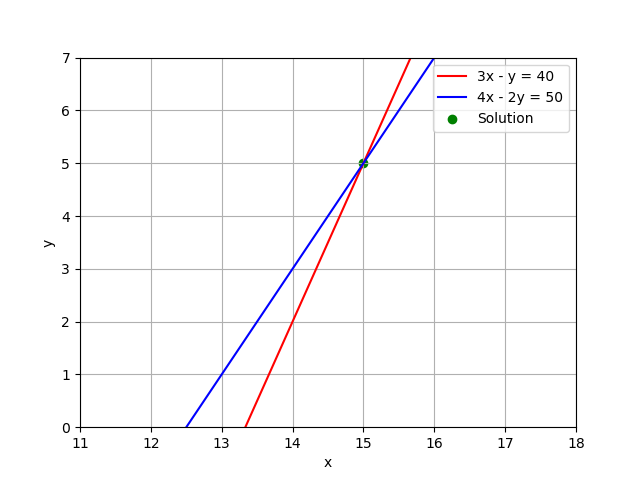
\includegraphics[width=0.8\columnwidth]{figs/fig.png}
  \caption{Solving the system: $3x - y = 40,\quad 4x - 2y = 50$.}
\end{figure}
\end{frame}

\end{document}

